\documentclass[MASTER.tex]{subfiles} 
\begin{document} 
 
 
 
 \huge
\[ \mbox{Other Interesting Python Packages} \]
 




 
 \begin{figure}
\centering

\includegraphics[width=0.7\linewidth]{SKL-logo}

\end{figure}

 
%===========================================================%

 
 \frametitle{scikit.learn}
  \begin{figure}
   \centering
   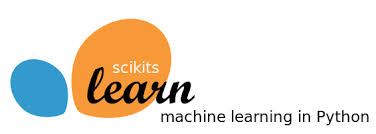
\includegraphics[width=0.5\linewidth]{SKL-logo2}
  
  \end{figure}
  
  
  scikit-learn is an open source machine learning library for the Python programming language. 
  scikit-learn features various classification, regression and clustering algorithms including support vector machines, logistic regression, naive Bayes, random forests, gradient boosting, k-means and DBSCAN.  scikit-learn is designed to interoperate with the Python numerical and scientific libraries NumPy and SciPy.
  
 
%===========================================================%
 
\textbf{Sci-Kit Learn Site info}
 \begin{figure}
\centering
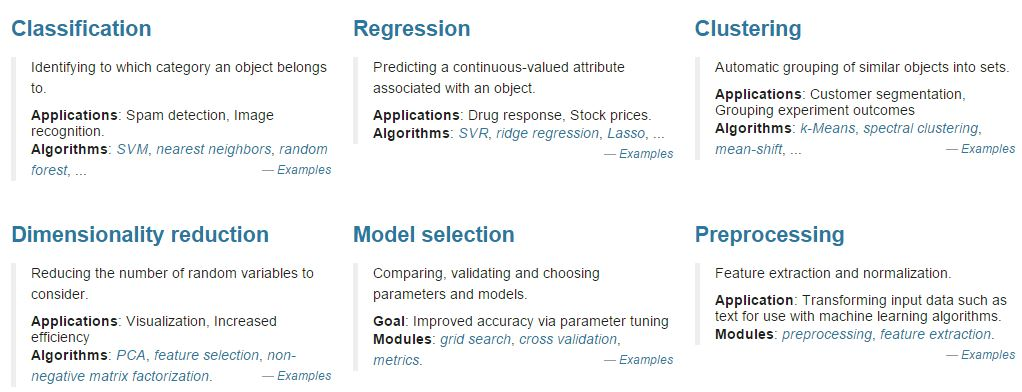
\includegraphics[width=1.1\linewidth]{SKLsiteinfo}
\end{figure}
 
%===========================================================%
 
\begin{figure}
\centering
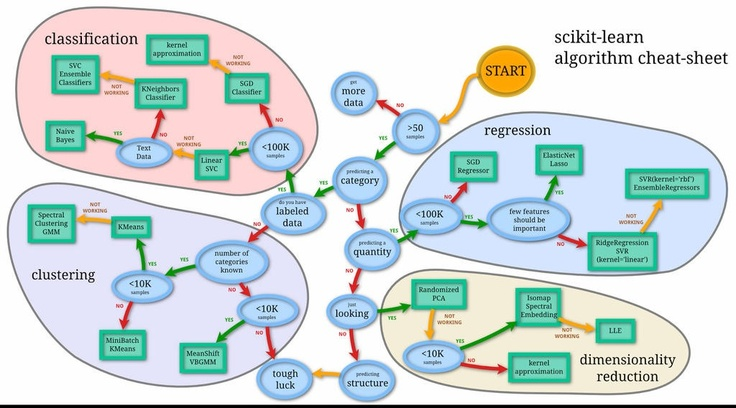
\includegraphics[width=0.9\linewidth]{SKLCheatSheet}

\end{figure}
 
%===========================================================%
 
 \begin{figure}
  \centering
  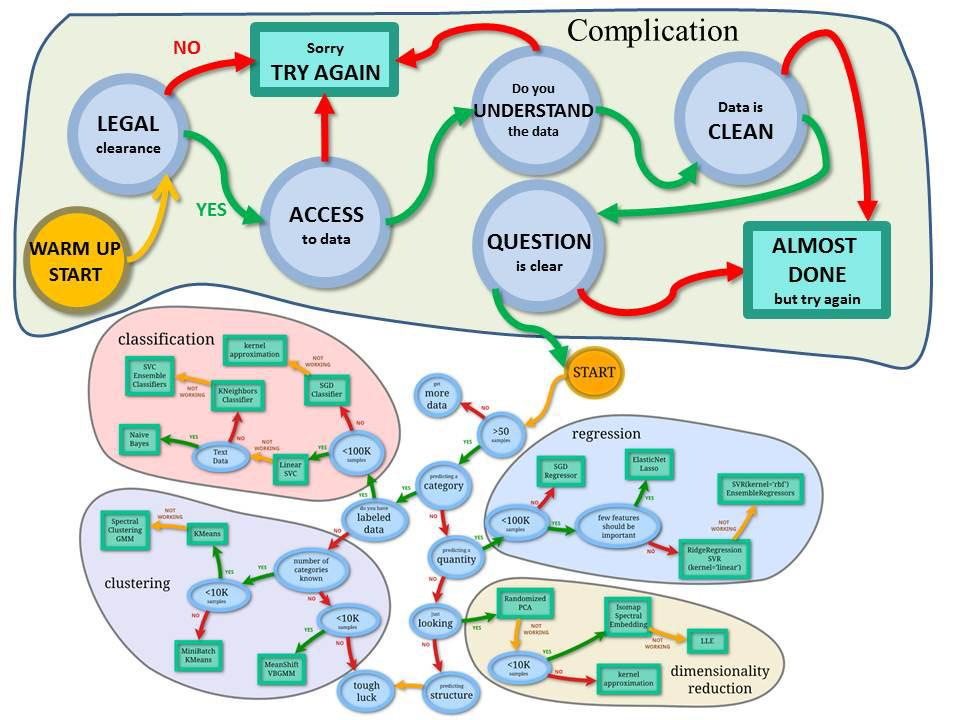
\includegraphics[width=0.9\linewidth]{SKLCheatSheet2}
  
 \end{figure}
 
%=========================================================== %
 
 \begin{figure}
\centering
\includegraphics[width=1.1\linewidth]{machinelearningquotes}
\end{figure}
  Machine Learning is statistics minus any checking of models or assumptions
 
%============================%
 
 \frametitle{The Data Science Profession}
 Data Science Retreat (Berlin)
 \begin{quote}
  MOOC have not  decreased the barrier of entry to machine-learning.
  
  
  Nowadays, you cannot be 'the guy who knows how to run (insert off-the-shelf-algo-here)'. 
  
  
  In dataland, that's the equivalent to being a code monkey. MOOCs and superb libraries (scikit-learn, R's ecosystem) made 
  sure there is plenty of people who can throw say a random forest to a problem. In the modern world, this is not adding that much value. 
 \end{quote}
 
%===========================================================%
 
\frametitle{Other Packages}
 
\textbf{pytz and babel}\\
ptyz and babel provide extended support for time zones and formatting information.\\ \bigskip
\textbf{rpy2 }\\
rpy2 provides an interface for calling R 3.0.x in Python, as well as facilities for easily moving data between
the two platforms.\\ \bigskip
\textbf{PyTables and h5py }\\
PyTables and h5py both provide access to HDF5 files, a flexible data storage format optimized for numeric
data.
 
\end{document}